\section{Modelando grafos en la memoria}

Ahora, la pregunta es como representamos un grafo en C++ y la respuesta es que no existe una única forma de hacer esto. Nosotros nos vamos a concentrar en los dos métodos más utilizados en la olimpiada.


\section{Matriz de adyacencia}

La matriz de adyacencia es una forma de representar un grafo que tal como indica su nombre, utiliza una matriz para esto.

La idea principal es tener una matriz de tamaño \(N\times N\) si tenemos \(N\) vértices. Ahora, si existe la arista \(\{i, j\}\), entonces \(matriz[i][j]=matriz[j][i]=1\). Caso contrario se tiene que \(matriz[i][j]=matriz[j][i]=0\).

Veamos un grafo y su matriz de adyacencia:

\begin{center}
	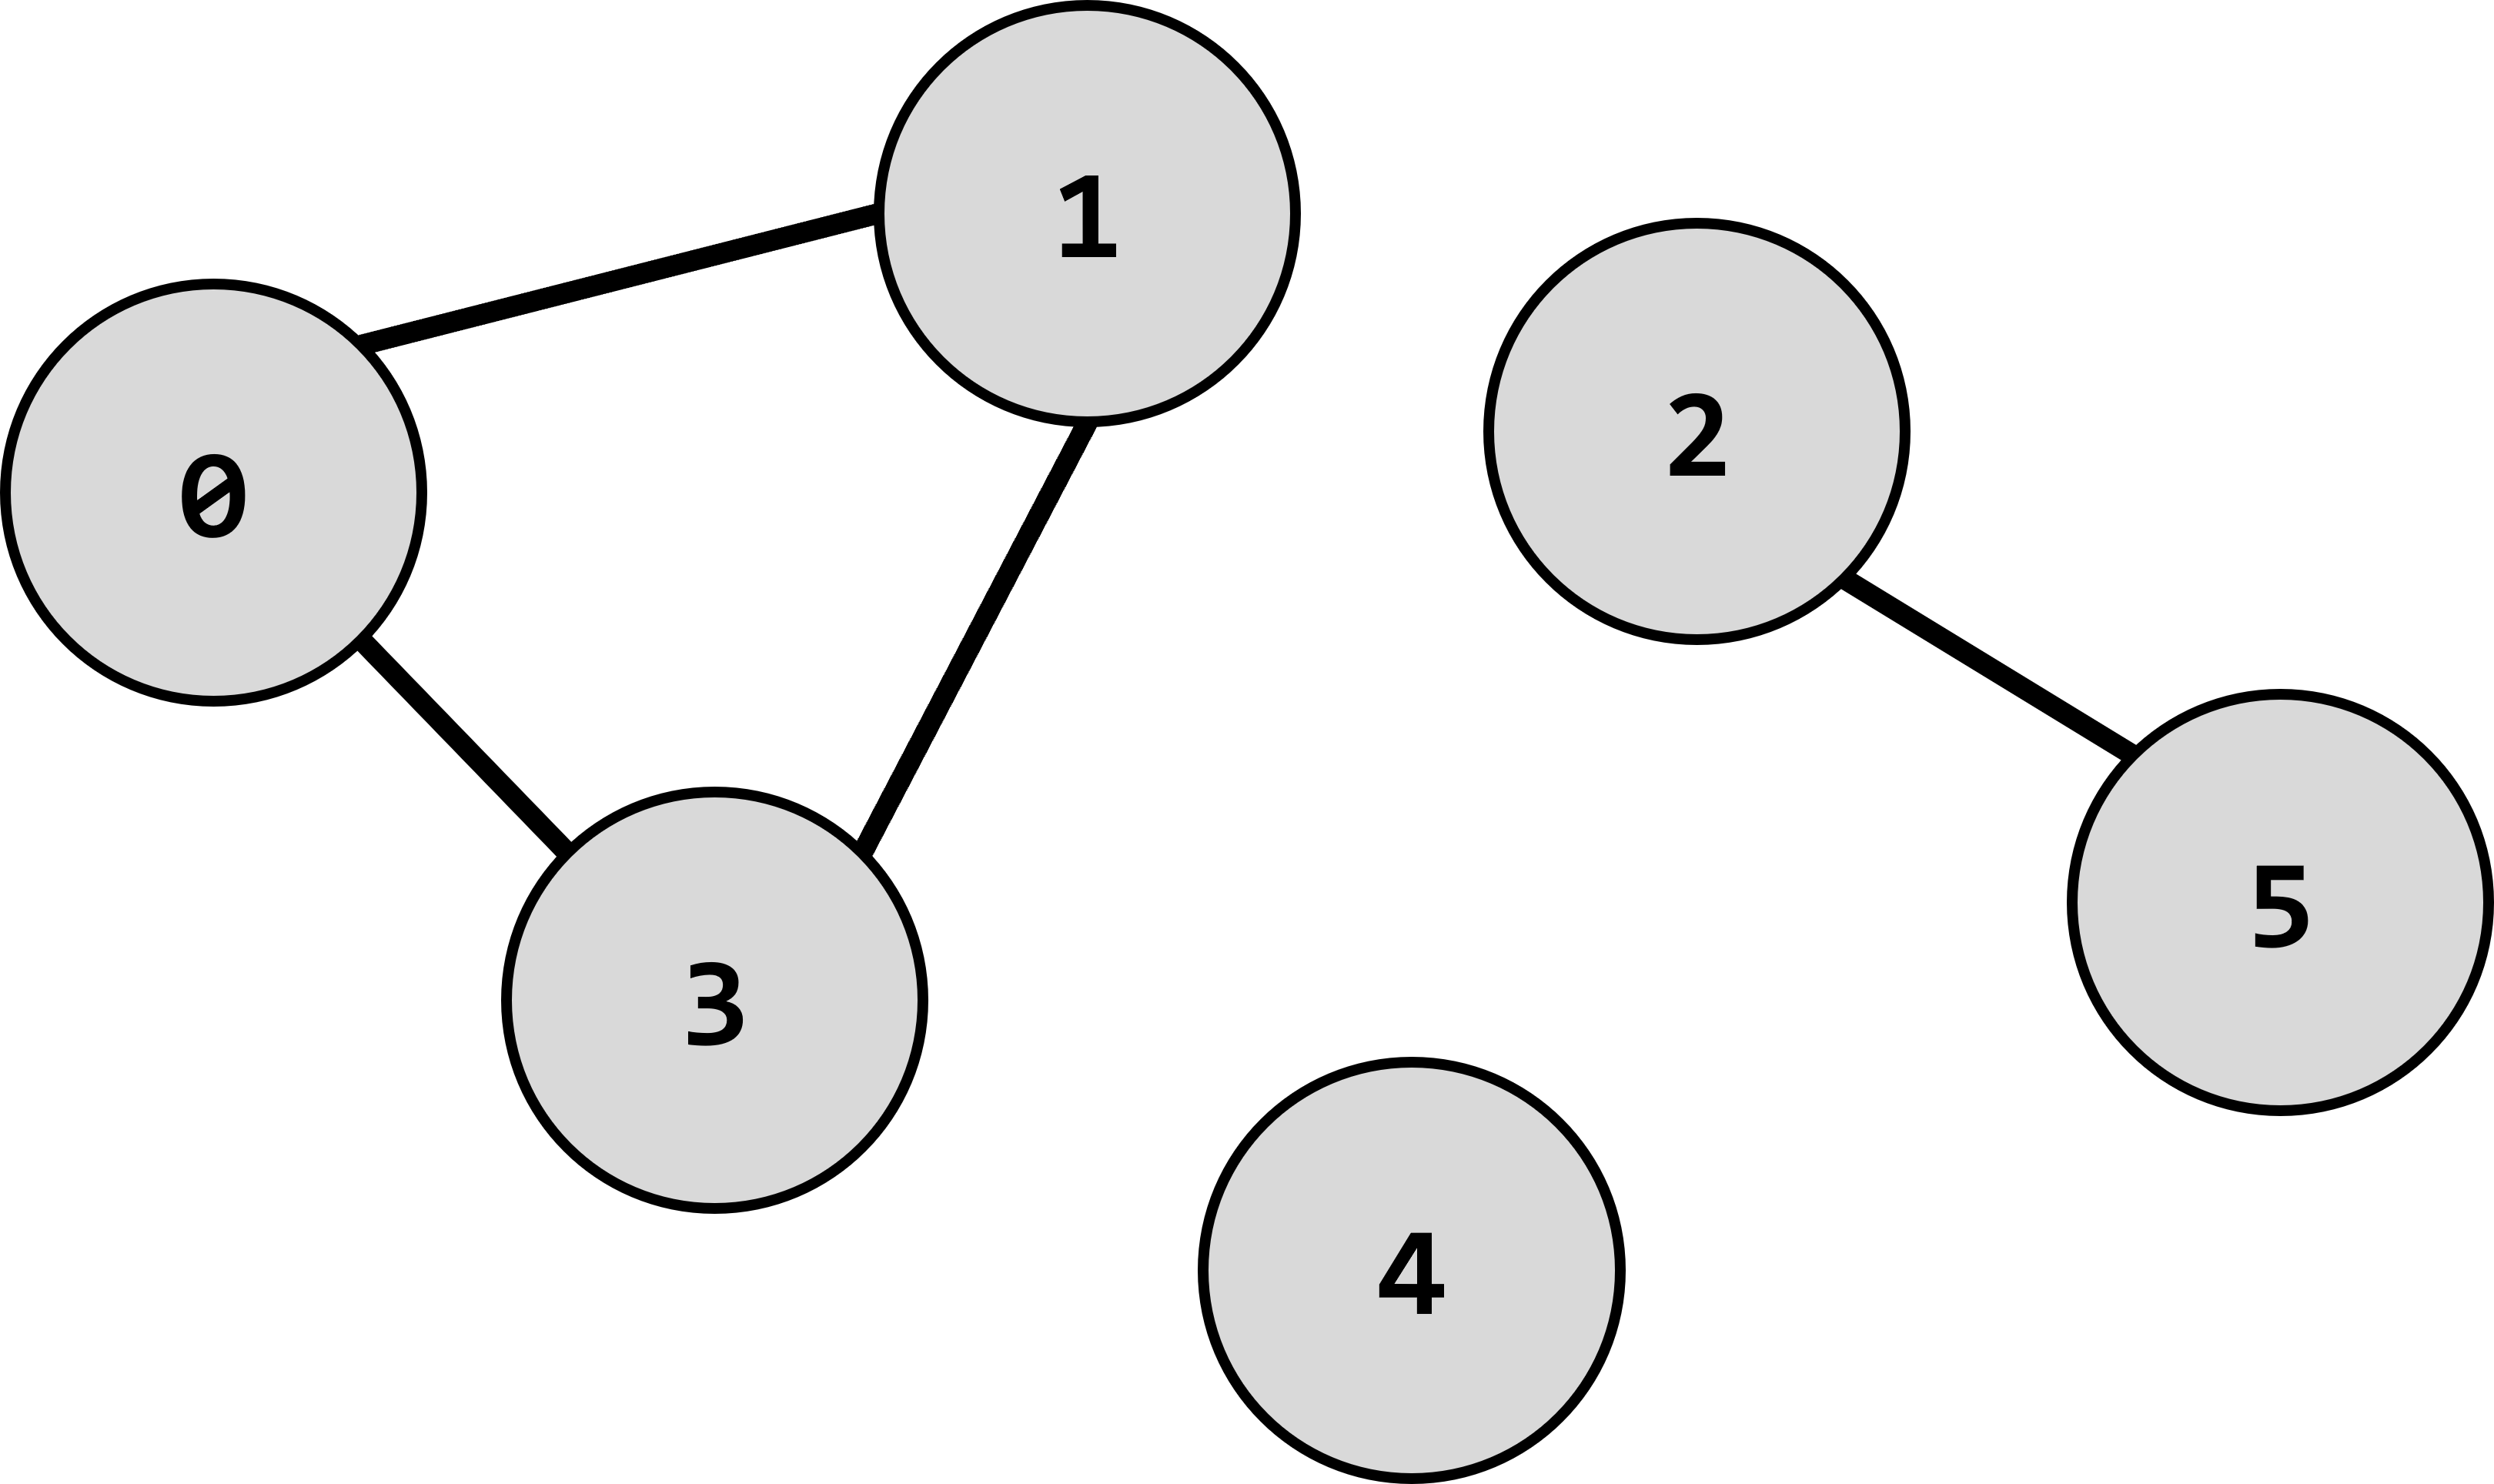
\includegraphics[scale=0.25]{grafos/grafo}
\end{center}
\begin{large}
	\begin{displaymath}	
		matriz = \begin{pmatrix}
			0 & 1 & 0 & 1 & 0 & 0\\
			1 & 0 & 0 & 1 & 0 & 0\\
			0 & 0 & 0 & 0 & 0 & 1\\
			1 & 1 & 0 & 0 & 0 & 0\\
			0 & 0 & 0 & 0 & 0 & 0\\
			0 & 0 & 1 & 0 & 0 & 0
		\end{pmatrix}
	\end{displaymath}
\end{large}

\begin{exercise}
	Un programa que pase de grupo de aristas a matriz.
\end{exercise}

\section{Lista de adyacencia}
Otra forma de representar un grafo es mediante el uso de una lista de adyacencia.

Este es el método principal que se usa en la olimpiada para grafos debido a su menor consumo de recursos.

Lo que hacemos es que para cada vértice guardamos una lista con sus vecinos. Veamos esto como se ve esto en el grafo anterior:
\begin{center}
	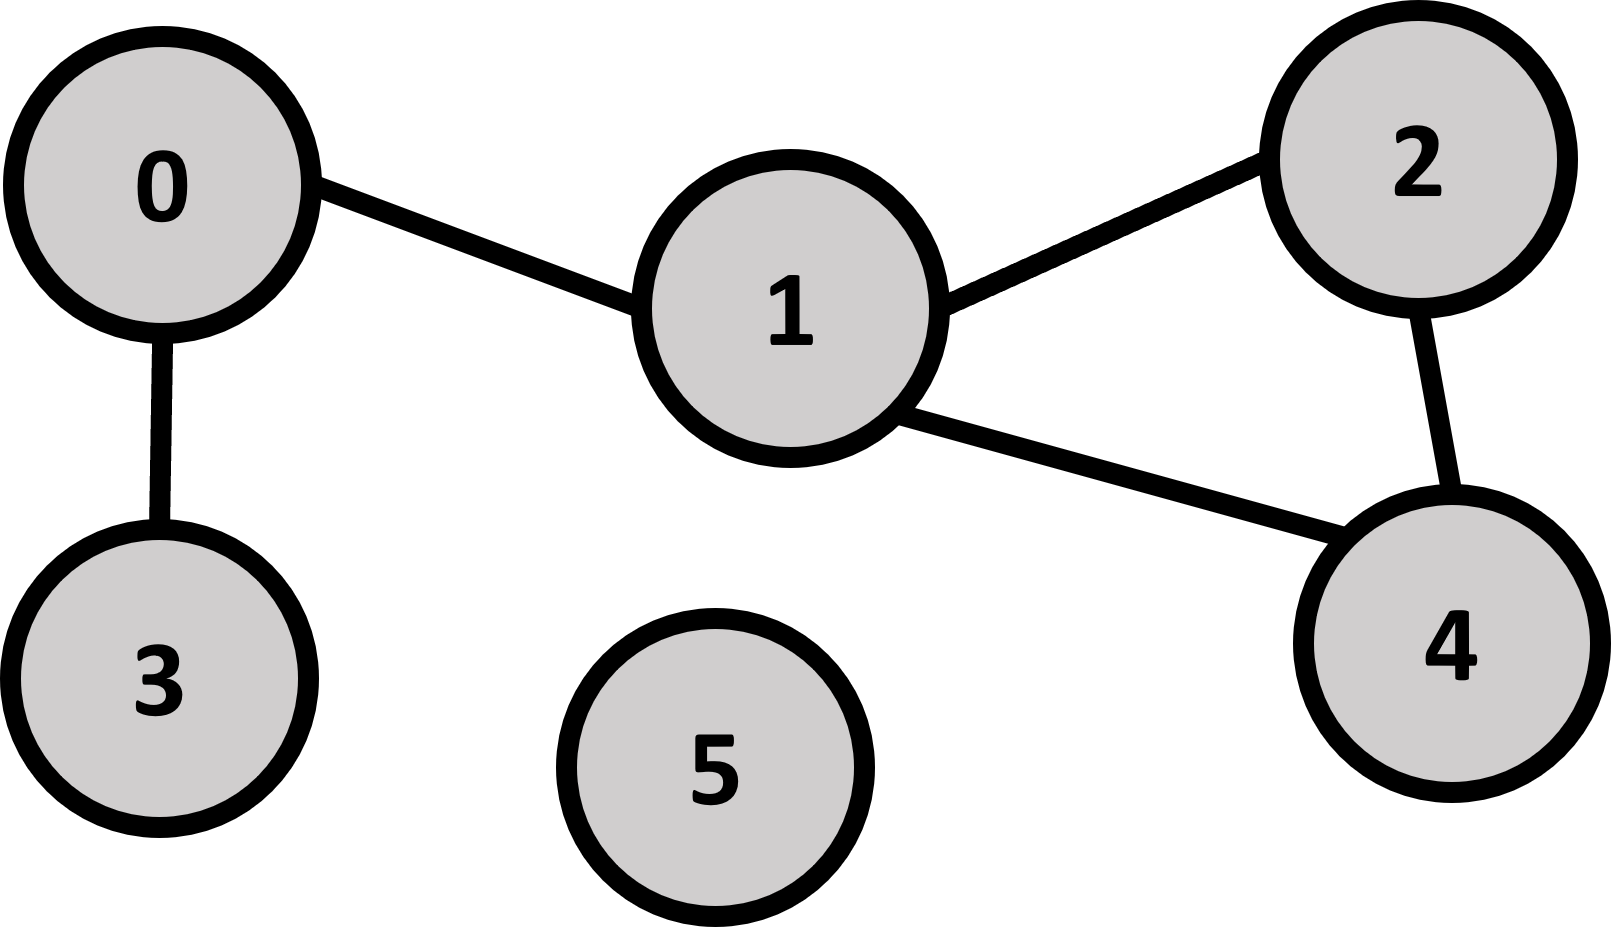
\includegraphics[scale=0.4]{grafos/grafo2}
\end{center}


{
\begin{align*}
listaAdyacencia[0] & =\{1,3\} \\
listaAdyacencia[1] & =\{2,0,4\}\\
listaAdyacencia[2] & =\{1,4\}\\
listaAdyacencia[3] & =\{0\}\\
listaAdyacencia[4] & =\{2,1\}\\
listaAdyacencia[5] & =\{ \}		
\end{align*}
}

Entonces, podemos ver que si existe la arista \(\{i,j\}\) entonces en la \verb|listaAdyacencia[i]| estará \verb|j|. Igualmente \verb|listaAdyacencia[j]| tendrá al valor de \verb|i|.

Para implementar esto utilizamos un arreglo de \lstinline|vector<int>| de la siguiente manera:

\begin{minipage}{\linewidth}
\begin{lstlisting}
//Tenemos 100050 vectores
vector<int> listaAdyacencia[100050];

int main() {
	listaAdyacencia[0].push_back(1);
	listaAdyacencia[0].push_back(3);
	listaAdyacencia[1].push_back(2);
	listaAdyacencia[1].push_back(0);
	listaAdyacencia[1].push_back(4);
	listaAdyacencia[2].push_back(1);
	listaAdyacencia[2].push_back(4);
	listaAdyacencia[3].push_back(0);
	listaAdyacencia[4].push_back(2);
	listaAdyacencia[4].push_back(1);
	cout << "TENEMOS EL GRAFO EN MEMORIA";
	return 0;
}
\end{lstlisting}
\end{minipage}

La principal ventaja de la lista de adyacencia sobre la matriz de adyacencia es que no gastamos memoria guardando tantos ceros. Esto gasta tanta una cantidad de memoria proporcional a la cantidad de aristas.

\begin{exercise}
	Dado un grafo, imprime la lista de adyacencia.
	
	TODO
\end{exercise}

